\subsection{Ca sử dụng xem thông tin chi tiết địa điểm du lịch}
\noindent Ca sử dụng này mô tả cách người dùng xem thông tin chi tiết về một địa điểm du lịch cụ thể, bao gồm mô tả, hình ảnh, địa chỉ, đánh giá và các địa điểm liên quan khác. Bảng~\ref{tab:uc_view_place_details_spec} trình bày chi tiết đặc tả ca sử dụng, bao gồm luồng sự kiện chính, các điều kiện và yêu cầu liên quan. Các biểu đồ hoạt động, quan hệ (Bảng~\ref{tab:uc_view_place_details_diagrams}) và tuần tự (Hình~\ref{fig:3-3-8-sequence-diagram}) minh họa rõ hơn về quy trình và tương tác hệ thống khi người dùng xem chi tiết địa điểm.
% \vspace{0.5cm} % Adjust spacing if needed

% Use longtable environment
% Need \usepackage{longtable} and \usepackage{calc} in preamble
\begin{longtable}{| p{4cm} | p{\dimexpr\linewidth-4cm-4\tabcolsep} |} % Adjust widths as needed
    \caption{Đặc tả ca sử dụng xem thông tin chi tiết địa điểm du lịch} % Caption inside longtable
    \label{tab:uc_view_place_details_spec} \\ % Label after caption

    \hline
    \textbf{Mô tả} & Người dùng xem chi tiết thông tin địa điểm du lịch. \\
    \hline
    \endfirsthead % Header for the first page

    % No \endhead content needed

    % No \endfoot content needed

    \hline % Footer for the last page
    \endlastfoot

    % --- Table Content ---
    \textbf{Luồng cơ bản} & 1. Người dùng bấm vào một địa điểm du lịch muốn xem thông tin (từ danh sách tìm kiếm, gợi ý, bản đồ, v.v.). \newline
                           2. Hệ thống lấy thông tin chi tiết của địa điểm từ cơ sở dữ liệu và các API bên ngoài (nếu cần). \newline
                           3. Hệ thống hiển thị thông tin chi tiết địa điểm du lịch bao gồm tên, mô tả, địa chỉ, số điện thoại, ảnh, đánh giá và các địa điểm liên quan. \\
    \hline
    % \textbf{Luồng thay thế} & (Nếu có luồng thay thế, ví dụ: địa điểm không tồn tại, lỗi API) \\
    % \hline
    \textbf{Tiền điều kiện} & Người dùng đang đăng nhập và phiên đăng nhập chưa kết thúc. \\
    \hline
    \textbf{Hậu điều kiện} & - Người dùng có thể xem thông tin về địa điểm như mô tả, địa chỉ, sđt, ảnh. \newline
                           - Người dùng có thể xem chi tiết các đánh giá về địa điểm. \newline
                           - Người dùng có thể xem chi tiết các địa điểm liên quan. \\
    \hline
    \textbf{Yêu cầu phi chức năng} & Hệ thống xử lý lấy và hiển thị thông tin không quá 2 giây. \\
    % --- End Table Content ---

\end{longtable}
\vspace{0.8cm}

\begin{table}[H] % Wrap the diagrams table
    \centering
    \caption{Biểu đồ hoạt động ca sử dụng xem thông tin chi tiết địa điểm du lịch} % Add caption
    \label{tab:uc_view_place_details_diagrams} % Add label
    \begin{tabular}{| c | c |}
        \hline
        \textbf{Biểu đồ hoạt động} & \textbf{Quan hệ} \\
        \hline
        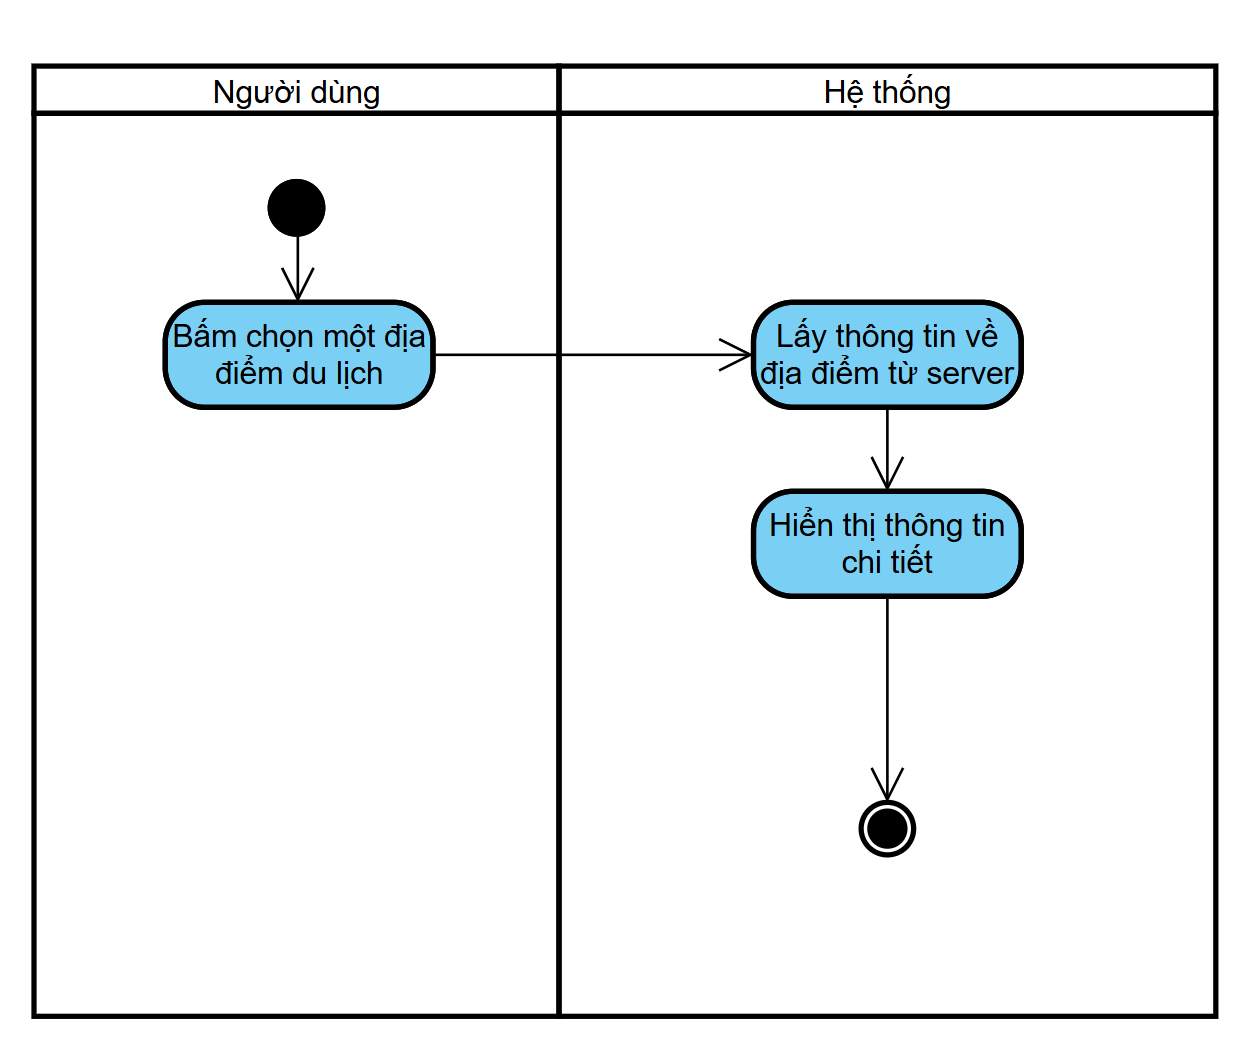
\includegraphics[width=0.5\linewidth]{figures/c3/3-3-8-ad.png} % Specified width
        &
        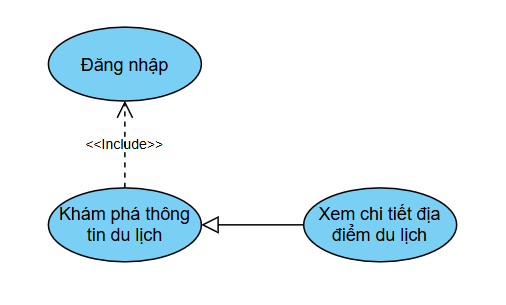
\includegraphics[width=0.45\linewidth]{figures/c3/3-3-8-rd.png} \\ % Specified width
        \hline
    \end{tabular}
\end{table}

\begin{figure}[H]
    \centering
    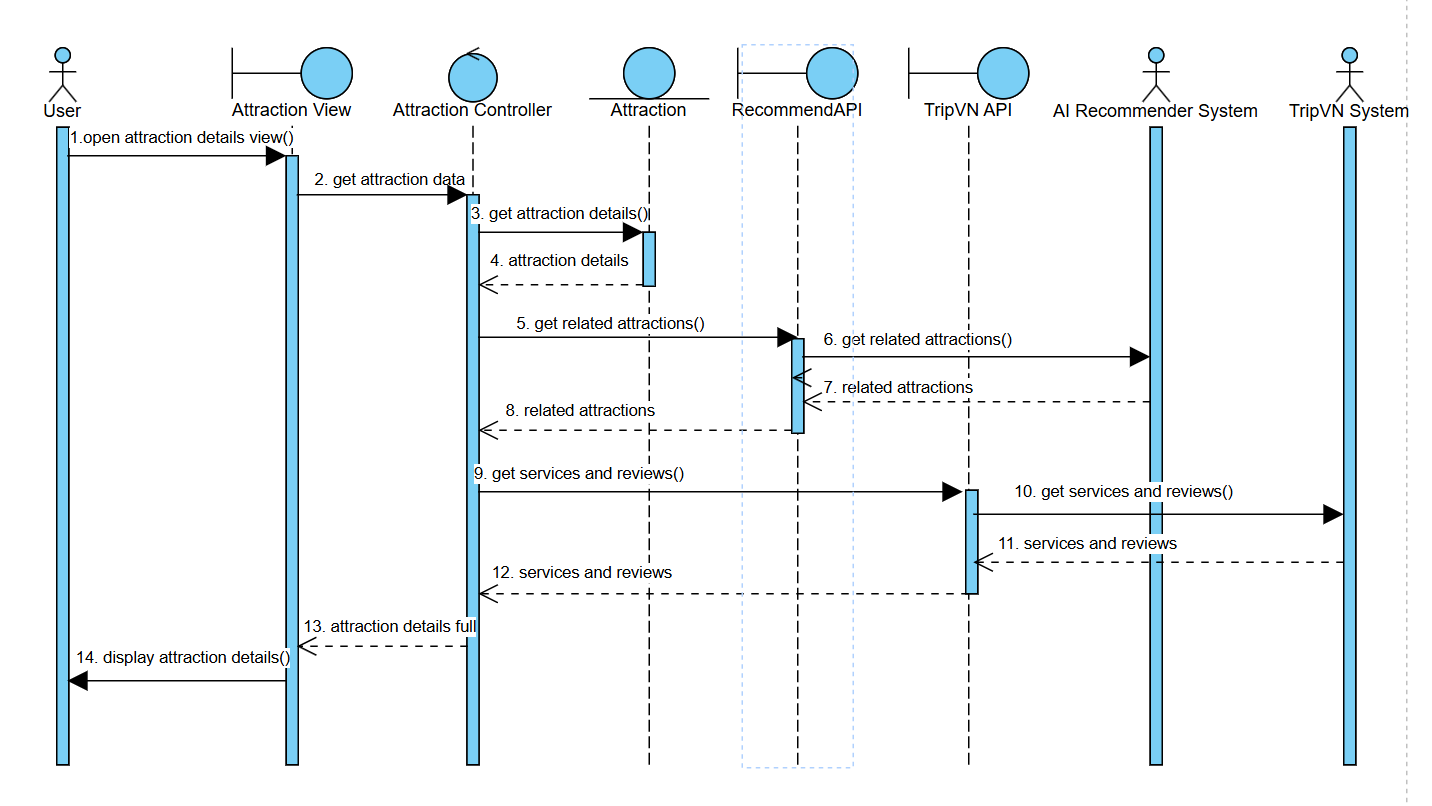
\includegraphics[width=1\textwidth]{figures/c3/3-3-8-sd.png} % Specified width
    \caption{Biểu đồ tuần tự ca sử dụng xem thông tin chi tiết địa điểm du lịch.}
    \label{fig:3-3-8-sequence-diagram}
\end{figure}